\documentclass{article}

% if you need to pass options to natbib, use, e.g.:
% \PassOptionsToPackage{numbers, compress}{natbib}
% before loading nips_2017
%

%\usepackage{nips_2017}

\usepackage[utf8]{inputenc} % allow utf-8 input
\usepackage[T1]{fontenc}    % use 8-bit T1 fonts

%%%%REFERENCING%%%%%
\usepackage[dvipsnames]{xcolor}
\usepackage{hyperref}
\hypersetup{
    colorlinks=true,
    linkcolor=Blue,
    filecolor=magenta,      
    urlcolor=OliveGreen,
    citecolor=Maroon,
}
\usepackage[capitalize,nameinlink,noabbrev]{cleveref}
\usepackage{autonum}
\usepackage{url}            % simple URL typesetting
\usepackage{booktabs}       % professional-quality tables
\usepackage{amsfonts}       % blackboard math symbols
\usepackage{nicefrac}       % compact symbols for 1/2, etc.
\usepackage{microtype}      % microtypography

\usepackage{subfigure}
\usepackage{amsmath,amsthm,amssymb,bbm}
\usepackage{graphicx}
\usepackage[T1]{fontenc}
\usepackage{verbatim}


\usepackage[final,nonatbib]{nips_2017}
\usepackage[style=numeric]{biblatex}
\bibliography{library}


\makeatletter
\catcode`! 3
\catcode0 12

% The update chooses safer macro names.

% It could be useful to allow #1 to be itself a macro expanding
% to some rows. One could replace \Mar@DoOneRow by 
% \expandafter\Mar@DoOneRow but then general usage must be aware
% of this one-expansion of contents.

% Usage: \Transpose { &-separated cells \\ &-separated cells \\ ...
%                     ...\\&-separated cells and *no* final \\ }

% Can be used inside amsmath matrices as well as inside LaTeX tabular's
% 
\def\Transpose #1{\romannumeral0\expandafter
                  \Mar@Transpose@a\romannumeral`^^@\Mar@DoOneRow #1\\!\\}

\def\Mar@DoOneRow #1\\{\Mar@DoOneRow@a {}#1&^^@&}%

\def\Mar@DoOneRow@a #1#2&{%
    \if^^@\detokenize{#2}\expandafter\@gobble\fi
    \Mar@DoOneRow@a {#1#2\\}%
}%

% unbraced #1 here will end in \\^^@\\
\def\Mar@Transpose@a #1#2\\{\ifx!#2\expandafter\Mar@FinishTranspose\fi
    \expandafter\Mar@Transpose@b\romannumeral`^^@\Mar@DoOneRow@a {}#2&^^@&#1}

% unbraced #1 here will end with \\^^@\\
% It represents a new transposed row with an extra ^^@ cell.
% The #2 here ends in \\. It holds the first already transposed rows.
\def\Mar@Transpose@b #1#2^^@\\{\Mar@Join {}#2^^@!#1}

% when #3=^^@ happens after #4\\ there is still ^^@\\
% update slightly simplifies \Mar@Join.
\def\Mar@Join #1#2\\#3!#4\\%
   {\if^^@\detokenize{#3}\expandafter\Mar@EndJoin\fi
    \Mar@Join {#1#2&#4\\}#3!}%

% unbraced #1 ends with \\
\def\Mar@EndJoin\Mar@Join #1^^@!^^@\\{\Mar@Transpose@a {#1^^@\\}}

\def\Mar@FinishTranspose
    #1&^^@&#2\\^^@\\{ #2}% the \\^^@\\ pattern helps removing a final \\

\catcode`! 12
\catcode0 15 % null character "invalid": this is default LaTeX setting.
\makeatother


%HMM figure
\usepackage{tikz}
\usepackage{caption}

\title{Predictive Policing of Vancouver Crime with Hidden Markov Models}

% The \author macro works with any number of authors. There are two
% commands used to separate the names and addresses of multiple
% authors: \And and \AND.
%
% Using \And between authors leaves it to LaTeX to determine where to
% break the lines. Using \AND forces a line break at that point. So,
% if LaTeX puts 3 of 4 authors names on the first line, and the last
% on the second line, try using \AND instead of \And before the third
% author name.

\author{
Cody Griffith \\
  Department of Mathematics\\
  The University of British Columbia\\
  \texttt{cgriff@math.ubc.ca} \\
 \And
   Ziming Yin \\
  Department of Mathematics\\
  The University of British Columbia\\
  \texttt{ziming@math.ubc.ca} \\
  \And
  Tim Jaschek \\
  Department of Mathematics \\
  The University of British Columbia\\
  \texttt{jaschekt@math.ubc.ca} \\
}

\begin{document}
% \nipsfinalcopy is no longer used

\maketitle

\begin{abstract}
 The aim of this work is to predict time and location of possible future crimes with unsupervised machine learning techniques. We generate a time-chain of GPS locations of likely crimes in the city of Vancouver with a hidden Markov model (HMM). As a training set we use data set consisting of different classes of crimes with time and location. The dataset contains more than half a million of entries and is publicly available.
Unfortunately We did not find crucial hidden states that would improve the prediction. However, a different initialization of our model might provide significantly better results.
\end{abstract}

\section{Introduction}
\label{sec:into}

\indent The path of predictive policing has taken many twists and turns in attempting to use ever increasingly large datasets to better allocate police resources. There are many fantastic examples of this being done successfully to help minimize local crime and agencies world wide have taken notice. An interesting model, called "\textit{Series Finder}" \cite{wang2013learning}, has the ability to detect crime patterns purely from data and has helped trained professionals to update their own database while also outperforming the competitors. However, this algorithm has not been applied on large scales yet.

In practice, most of the available predictive policing tools are concerned with predicting areas where crimes are most likely to happen. Although big companies like IBM offer predictive policing tools, one of the most widely deployed products comes from a small Santa Cruz, Calif. firm called "\textit{PredPol}" \cite{huff}. According to the company's website their algorithm is based on machine-learning and is cities including Los Angeles, Chicago and Atlanta, but due to licensing and proprietary issues, we aren't sure what techniques are being done.

Here in Vancouver, the first city in Canada to attempt predictive policing, a software called "\textit{GeoDash}" \cite{geo} gives real-time updates to patrolling officers for when and where crimes have occurred for nearby homes. This software is more than just an accessible database though, as it has the ability to also allocate officer time by forming a heat map of for future break-ins with probabilistic methods. This of course leads to prevented crime as well as optimizing police funding and public safety.
Even though they do not discuss machine learning aspects, we would like to point out the works of 
\cite{viz1} and \cite{viz2}, which provide helpful visualizations of crime data in Vancouver.

More examples for the applications of machine learning to crime data can be found 
in \cite{mcclendon2015using}, where linear regression, additive regression and decision stumps are used,
in \cite{kang2017prediction}, where a deep neural network is fitted to crime data 
and \cite{hidden}, whoses authors follow a similar strategy to ours by constructing a hidden Markov model.


Although, there is never good without bad and there have been failures of predictive policing. The most famous example was in Los Angeles where a model had begun to be used but it had been trained on racially profiled data. Thus, the model began to racially profile and the department had the luxury of pointing the finger at a computer when a minority was treated with injustice. Aspects of biased arrests are discussed in the paper \cite{racism}. What must be taken from this is not that Machine Learning and Policing should not be mixed, rather that this area is extremely sensitive and models need to be built on data that is pure in intent. For the purposes of all models mentioned above, \textit{Series Finder}, \textit{GeoDash} and the tools of \textit{PredPol}, human specific data was not used in any point of the learning or training of the model. It is here that we take inspiration and apply this to our own model.

We were unable to find algorithm-specific approaches to the \textit{GeoDash} model for proprietary reasons, this also is a much more cumbersome project with entire data warehouses and multi-stream project pipelines that would be impossible for three poor graduate students to replicate. Instead, we consider applying a Hidden Markov Model (HMM) to open source data that can be found at \cite{Dataset} with the aim to both forecast future crime and isolate location of crime within Vancouver, British Columbia. We choose to use an HMM as we are not criminal analysts and have no keen eye for spotting patterns within data, instead we hope to train an HMM to find hidden clusters and interdependences for us to better predict the future. 

\section{Exploratory Data Analysis}
\label{sec:stats}

The dataset we used is publicly available and weekly updated by the Vancouver Police Department \cite{Dataset}. It is roughly 30MB in size and contains information on the type of crime (i.e theft, breaking and entering, etc.), time (i.e year, day, hour and minute) and the coordinate of crime (i.e X and Y). This dataset goes as far back as 2003 and has a total of over 500,000 entries. From a simple exploratory search seen in \cref{fig:exploratory_data}, we consider the histogram of frequencies across the various time scales. The following conclusions are made;
\begin{itemize}
\item  Across years in \cref{fig:typeyear} we notice here that there is a spike in almost all types of crime for 2008 and following that a steady decrease in most until another rise in 2013. We do not know the reason for the peak in 2008. Surprisingly neither the Vancouver Olympic Games 2010 nor the Vancouver Stanley Cup riots from 2011 had a significant effect on the number of crimes committed in the year.
\item Across months in \cref{fig:typemonth} all types of crime seem to be near constant for each month.
\item Across days in \cref{fig:typeday} we have that day 31 doesn't happen for ever month so it is noticeably lower in count. Small spikes seem to occur near the middle of the month, but everything is rather uniform. 
\item Across hours in \cref{fig:typehour} we find the most interesting behavior. All types seems to behavior rather erratically with the general trend that crime seems to happen either early morning or late at night.
\end{itemize}

From our analysis, it becomes clear that we should consider to model at the hour scale as most other time scales are close to uniform in nature and thereby would not result in an interesting model. The hour scale on the other hand is best in two key ways: there is clearly some behavior that varies between crimes and across hours to present a complex interaction and there is realistic and practical value in having a model of crime on the hour. This could result in using police resource effectively and accurately or even to promote public safety in an interactive way.

\begin{figure}[h!]
\centering    
\subfigure[type by year]{\label{fig:typeyear}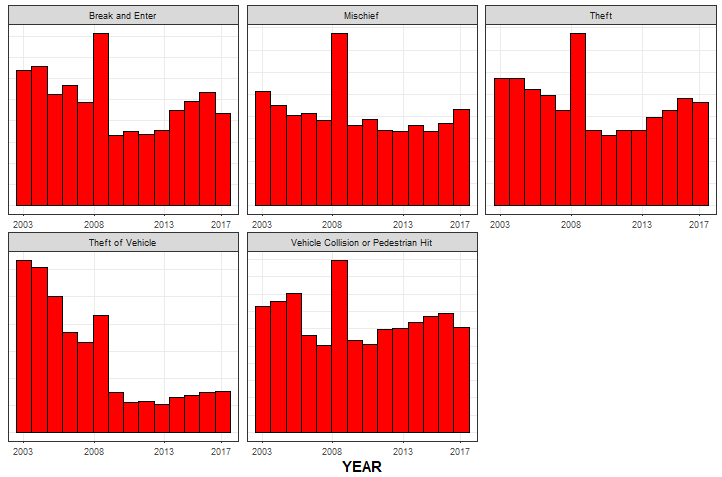
\includegraphics[width=.49\linewidth]{stats/type_vs_year.png}}
\subfigure[type by month]{\label{fig:typemonth}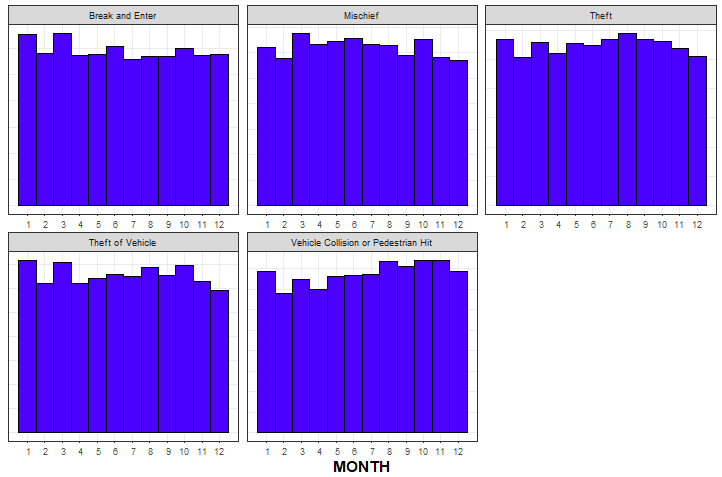
\includegraphics[width=.49\linewidth]{stats/type_vs_month.png}}
\subfigure[type by day]{\label{fig:typeday}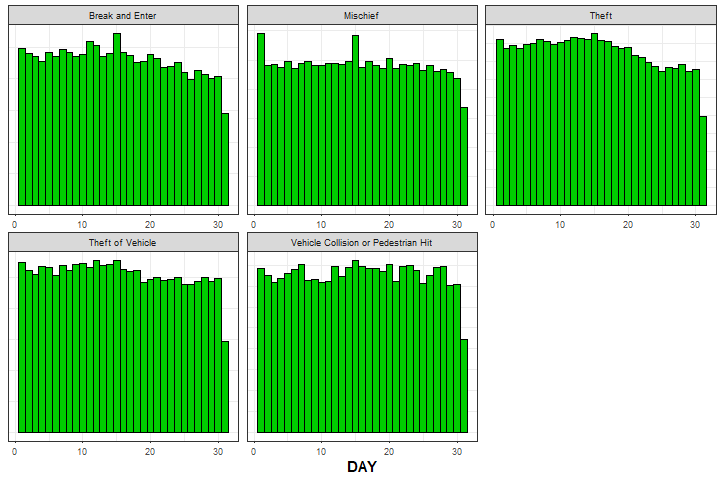
\includegraphics[width=.49\linewidth]{stats/type_vs_day.png}}
\subfigure[type by hour]{\label{fig:typehour}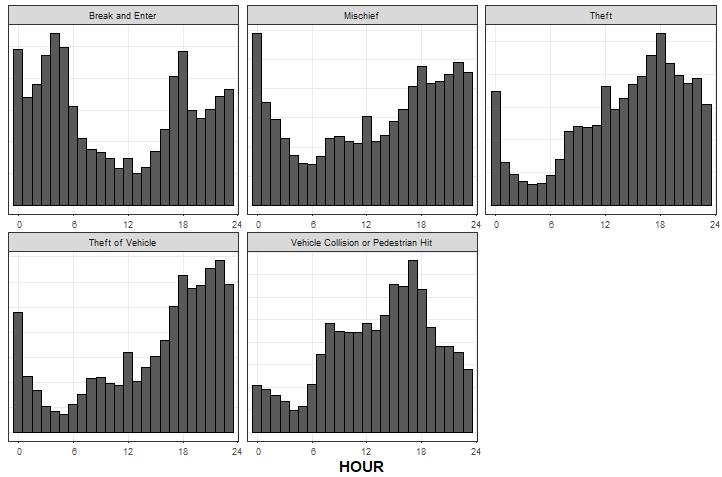
\includegraphics[width=.49\linewidth]{stats/type_vs_hour.png}}
\caption{Histogram data on each time scale with regard to each type of crime.}
\label{fig:exploratory_data}
\end{figure}

\section{Structuring the data}
According to GPS positions, we divided the city of Vancouver in a grid consisting of $13 \times 15$ cells. We decided to run a HMM for each of the cells separately.

For a fixed cell, we organized the data in the form of a four dimensional array, containing in the first component the type of crime, in the second component the number of the example and a (days)$\times$(hours) in the last components. Since the days 29-31 do not appear in every month we did not consider them. We have approximately 180 examples for the (days)$\times$(hours) matrices for each crime.


\section{Hidden Markov Model}
\label{sec:HMM}

The complexities of the types of crime, the hourly variability and spatial dependence in the data easily escape the untrained eye. We choose to use a Hidden Markov Model (HMM) to try to capture unknown patterns. 

An HMM is a directed acyclic graph (DAG) of a specific structure, that assumes that there is a hidden, unobserved Markov chain $\lbrace Z_i: i \in \mathbb{N}_0 \rbrace$  according to which the distribution of the actual observations $x_i$ is determined. \cref{HMM} visualizes the DAG corresponding to an HMM. Our main reference for hidden Markov models was \cite{hmc:em:baum}.


Let $(\Omega,\mathcal{F},\mathbb{P})$ be a probability space and consider a homogeneous hidden Markov chain $Z=\{Z_i\}_{i\in \mathbb{N}}$ and an observation process $X=\{X_i\}_{i\in\mathbb{N}}$, which are collections of the random variables
\begin{align}
Z_i: \quad &\Omega \rightarrow E \\
X_i: \quad &\Omega \rightarrow \mathbb{N}_{< c},
\end{align}
where $E$ denotes an abstract state space with $\vert E \vert =k$ and $\mathbb{N}_{<c}= \lbrace x \in \mathbb{N}_0 : x < c \rbrace$.
The hidden Markov chain is characterized by it's initial distribution $\pi \in \mathbb{R}^k$ and it's transition matrix, which we denote by $A \in \mathbb{R}^{k \times k}$. The variables of the observation process follow a categorical distribution according to the values of the corresponding hidden variables. We denote the emission matrix by $B \in \mathbb{R}^{k \times c}$.  As common in machine learning, recalling that we have a homogeneous Markov chain, we use the abbreviation $\mathbb{P}(X_i=x_i) = p(x_i)$ and extend it to multiple events. Note at this point that our model is homogeneous, otherwise we would have to learn the significantly more complex set of parameters 
$\hat{\Theta}= (\pi,A_1,\ldots ,A_T,B_1,\ldots, B_T)$. This simplifies our model but leaves room for improvement.

The interference of the DAG is given by
\begin{equation}
p(x_0,\dots,x_T,z_0,\dots,z_T) =
p(z_0) \prod_{t=0}^T p(x_t|z_{t}) \prod_{t=1}^T p(z_t|z_{t-1}).
\end{equation}
Given the data, we want our model to \emph{learn} the optimal choice of our model parameters $\Theta = (\pi,A,B)$. However, as half of our random variables are unobserved, we can not perform a standard maximum likelihood estimation. The machine learning technique of expectation maximization (EM) helps out. Instead of maximizing the negative log-likelihood (NLL) we randomly pick initial parameters and maximize the expected NLL with respect to these parameters. As \cite{in1}
and \cite{in2} showed, the algorithm is highly sensitive to it's initialization. We discuss this later on in more detail. 

In a more algorithmic fashion this can be denoted by
\begin{align}
\Theta^{(0)} & = (\pi^{(0)},A^{(0)},B^{(0)}) \\
\Theta^{(\ell+1)} &= \underset{\Theta}{\textup{arg\. max}} \, Q(\Theta^{(\ell)},\Theta), 
\end{align}
where for given realizations $\mathcal{X},\mathcal{Z}$ of $X$ and $Z$ of length $T$ (sampled according to $\Theta^{(\ell)}$) the function $Q$ is computed by
\begin{equation}
\label{eq:1}
Q(\Theta^{(\ell)},\Theta) = \mathbb{E}_{\mathcal{Z}|\mathcal{X},\Theta^{(\ell)}} \left[ \log(p(\mathcal{X},\mathcal{Z}|\Theta) \right] = \sum_\mathcal{Z} p(\mathcal{Z}|\mathcal{X},\Theta^{(\ell)}) \log(p(\mathcal{X},\mathcal{Z}|\Theta)).
\end{equation}
Using the fact that $p(\mathcal{X},\mathcal{Z}|\Theta)
=
\pi_{x_0} \prod_{t=1}^T a_{z_{t-1},z_t} \prod_{t=0}^T b_{z_{t},x_t} $ the logarithm on the ride hand side of \eqref{eq:1} splits into three terms. Therefore
\begin{align}
\label{eq:2}
Q(\Theta^{(\ell)},\Theta) = \sum_\mathcal{Z} & \log(\pi_{x_0}) p(\mathcal{Z}|\mathcal{X},\Theta^{(\ell)}) 
+
\sum_\mathcal{Z} \sum_{t=0}^T \log(b_{z_{t},x_t}) p(\mathcal{Z}|\mathcal{X},\Theta^{(\ell)})\\ 
&+
\sum_\mathcal{Z} \sum_{t=1}^T \log(a_{z_{t-1},z_t}) p(\mathcal{Z}|\mathcal{X},\Theta^{(\ell)}). 
\end{align}
To find the argmax one can now use the structure of the DAG and the resulting conditional independences to compute the terms $p(z_t|\mathcal{X},\Theta^{(\ell)})$ and optimize each term of \eqref{eq:2} with methods of multivariate calculus. This yields the EM-updates
\begin{align}
\pi^{(\ell+1)}_i &= \frac{p(\mathcal{X},z_0=e_i | \Theta^{(\ell)})}{p(\mathcal{X},\Theta^{(\ell)})} \\
a^{(\ell+1)}_{ij} &= \frac{\sum_{t=1}^T p(\mathcal{X},z_{t-1}=e_i,z_t=e_j | \Theta^{(\ell)})}{\sum_{t=1}^T p(\mathcal{X},z_{t-1}=e_i| \Theta^{(\ell)})} \\
b^{(\ell+1)}_{ij} &= \frac{\sum_{t=1}^T p(\mathcal{X},z_t=e_i | \Theta^{(\ell)}) \delta_{x_t,j}}{\sum_{t=1}^T p(\mathcal{X},z_t=e_i| \Theta^{(\ell)})} .
\end{align}
For efficient computation the forward-backward algorithm can be used. This procedure is also known as the Baum-Welch algorithm. An excellent reference for the Baum-Welch algorithm and it's relation to EM provides \cite{baumwelch}.



\begin{figure}
\centering
\begin{tikzpicture}
 	\foreach \x in {0,...,5}{
		\draw[fill=orange,opacity=.3] (2*\x,2) circle (.4cm);
        \draw (2*\x,2) node{$Z_\x$};
        \draw (2*\x,0) circle (.4cm) node{$X_\x$}; 
        \draw[->] (2*\x,1.6) -- (2*\x,0.45);    
        }
	\foreach \x in {0,...,4}{ 
        \draw[->] (2*\x+0.4,2) -- (2*\x+1.55,2);   
        }
    \draw[->,dashed] (10+0.4,2) -- (10+1.55,2);
\end{tikzpicture}
\caption{Directed acyclig graph (DAG) corresponding to a hidden Markov model (HMM)}
\label{HMM}
\end{figure}

\section{Results}

Random samples of our HMM for two specific classes of crimes can be seen in
\cref{mischief}
and
\cref{car}. Our model has learned the distribution of the data very well. Especially when summing up the total amount of crimes committed within the duration of a month, the model seems to perform excellent.
However, once less data is given the similarity of prediction and reality is less impressive, which is consistent with the philosophy of the famous law of large numbers.

The significance of our HMM is not to find the area where over time most of the crimes where committed. In fact, a simple averaging model would probably outperform ours when just focusing on the data of the past. What we are interested in is whether there where hidden patterns discovered or not. The answer to this question is found in the matrix $B$, which tells us how likely it is to see a crime at a fixed location when the hidden chain $Z$ is in a fixed state.

Unfortunately we had to discover that our hidden states don't give an advantage when we try to predict a crime. The rows of matrix $B$ are almost identical. For example, with $k=10$ we obtained for a specific GPS box the transition matrix

\tiny{
\begin{equation}
B = 
\begin{bmatrix} \Transpose{
 .9929  &.007099 \\
 .9928  &.007102 \\
 .9929  &.007098\\
 .9929  &.007099 \\
 .9929  &.007069\\
 .9928  &.007103 \\
 .9929  &.007082 \\
 .9928  &.007107\\
 .9928  &.007110\\
 .9929  &.007074}
\end{bmatrix}
\end{equation}}

\normalsize
Even worse, the matrix $A$ that corresponds to the transition probabilities of the hidden Markov chain heavily depends on the initial conditions. Whenever we re-run our algorithm the matrix looks completely different. We already mentioned that \cite{in1} and \cite{in2} found that this is a problem of HMM in general. Unfortunately we did not have enough time to implement their suggestions for an optimal initialization. 


\begin{figure}
\centering    
\subfigure[Prediction for a month]
{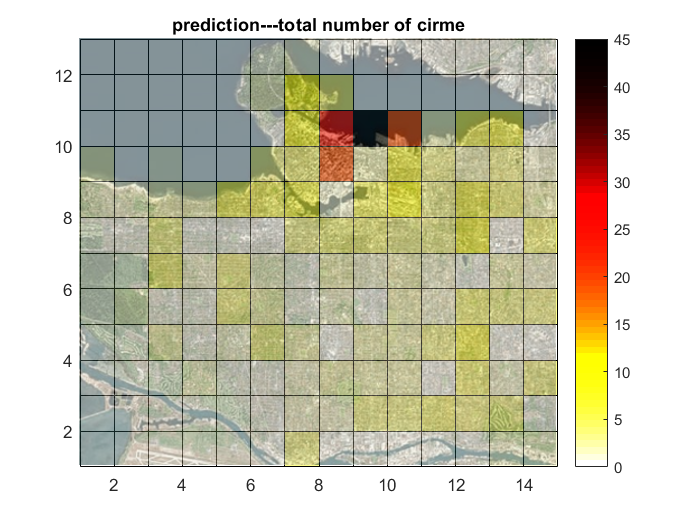
\includegraphics[width=.49\textwidth]{Images/predict.png}}
\subfigure[Reality for a month]
{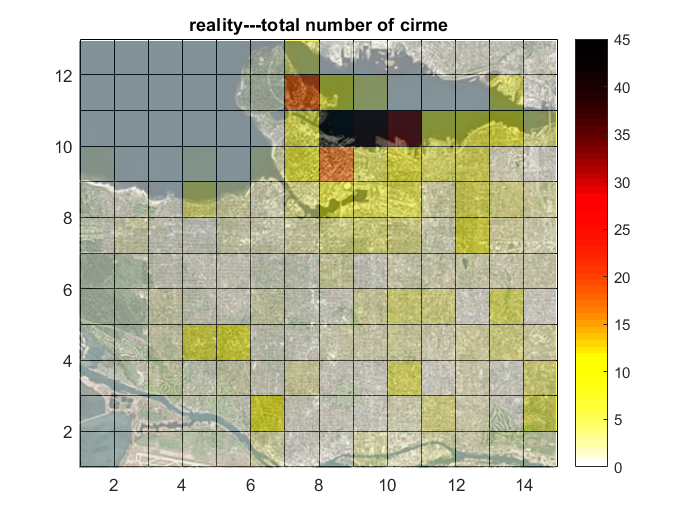
\includegraphics[width=.49\textwidth]{Images/real.png}}
\subfigure[Prediction for a day]
{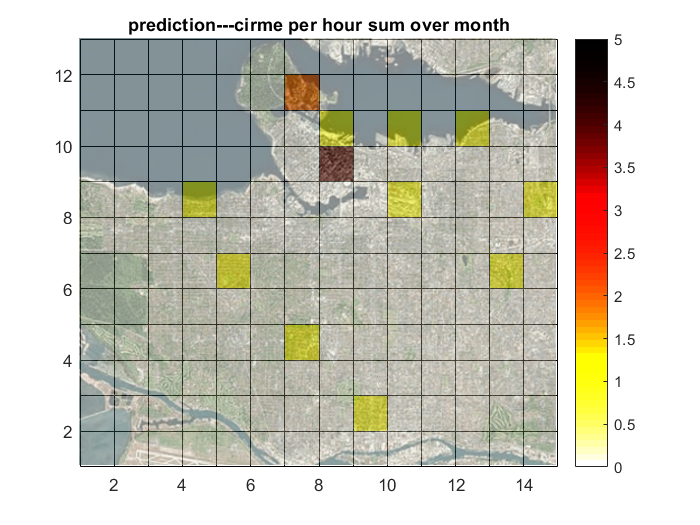
\includegraphics[width=.49\textwidth]{Images/predict2hour.png}}
\subfigure[Reality for a day]
{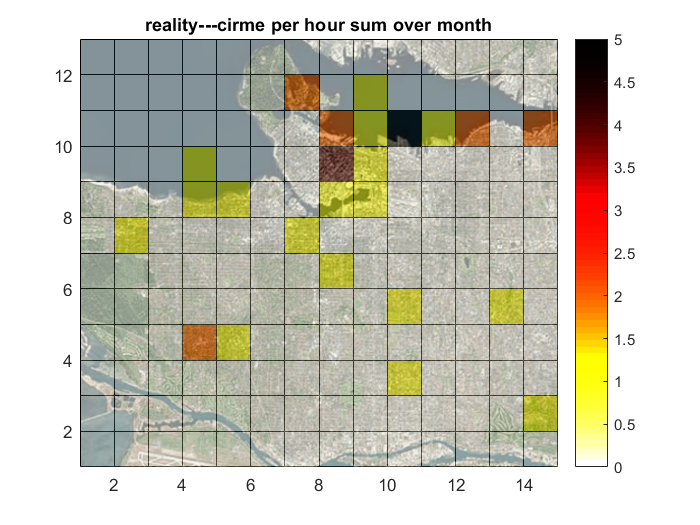
\includegraphics[width=.49\textwidth]{Images/real2hour.png}}
\caption{Results of our model for the crime: \emph{mischief}.}
\label{mischief}
\end{figure}

\begin{figure}
\centering    
\subfigure[Prediction for a month]
{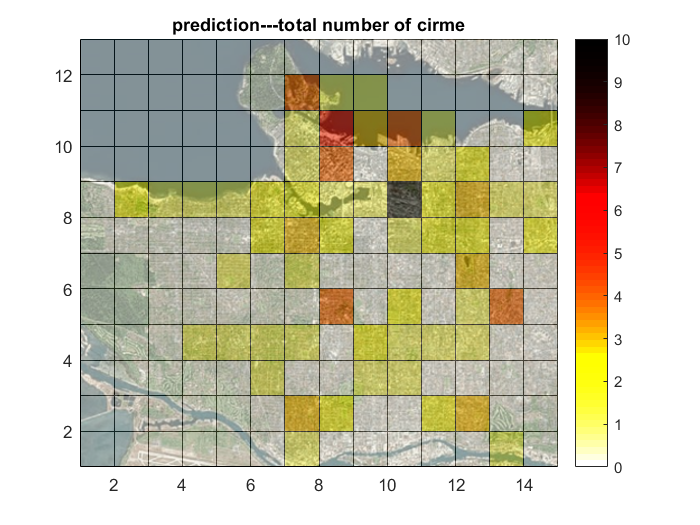
\includegraphics[width=.49\textwidth]{Images/predict5.png}}
\subfigure[Reality for a month]
{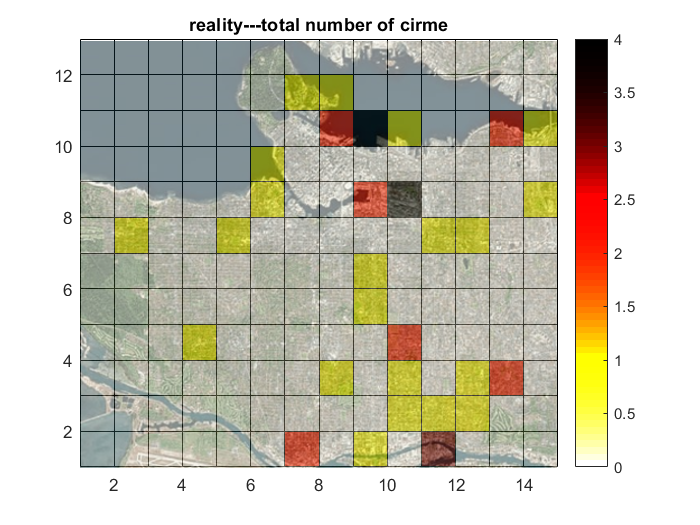
\includegraphics[width=.49\textwidth]{Images/real5.png}}
\subfigure[Prediction for a day]
{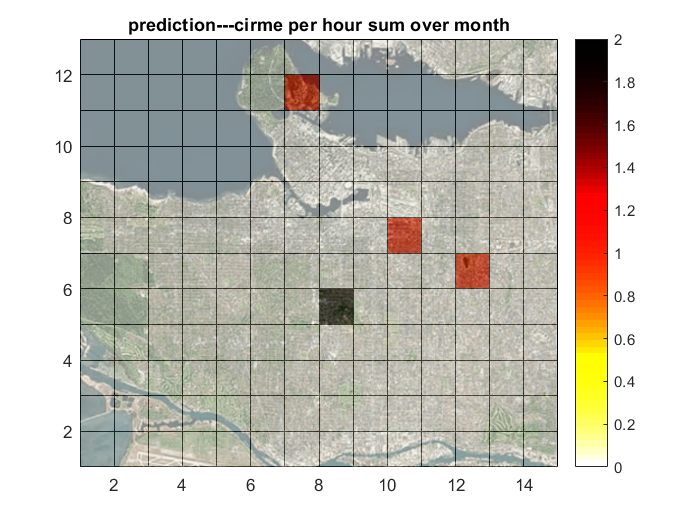
\includegraphics[width=.49\textwidth]{Images/predict5hour.png}}
\subfigure[Reality for a day]
{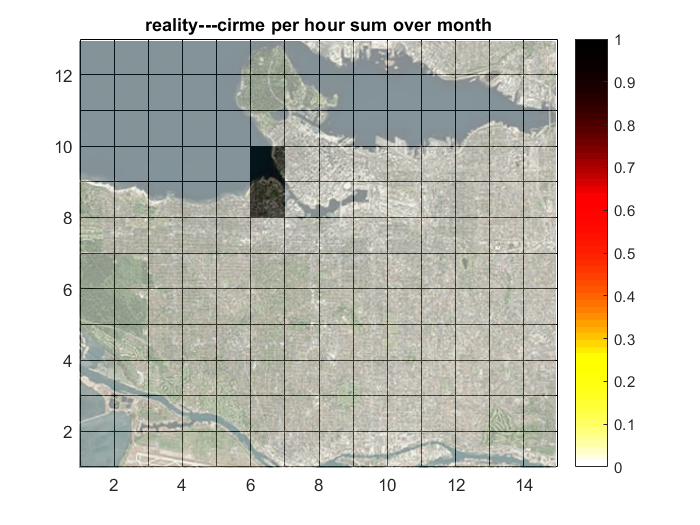
\includegraphics[width=.49\textwidth]{Images/real5hour.png}}
\caption{Results of our model for the crime: \emph{vehicle collision or pedestrian hit}.}
\label{car}
\end{figure}


\section{Future Work \& Conclusions}
\label{sec:FWC}

This work contributed to the research in predictive policing by implementing a model that has not yet been explored in this context. 

Our model in its current form should not be applied for predictive policing. It might send the police to wrong locations and does not provide an advantage when compared to a simple averaging.

However, we believe that the prediction of our model could be greatly improved by following an inhomogeneous strategy. Due to the limitations of time we where not able to implement such a model.

Furthermore, instead of sampling the $x_i$ from the $z_i$ according to a categorical distribution it might make sense to sample them with respect to a Poisson distribution. This would be reasonable as the decision of a criminal to commit a crime can be assumed to be Binomial distributed and as there are thousands of potential criminals. The natural limit of the Binomial distribution is the Poisson distribution . This would also have the advantage that there could be an arbitrary large number of crimes predicted (of course not in practice due to the limitations of the data types).

Another promising approach might be to use a conditional random field (CRF) or a more general restricted Bolzmann machine (RBM), where the dependencies between the hidden variables are  more complex. 



\subsubsection*{Acknowledgments}

We would like to thank the Vancouver Police department for providing the data set that was used in our project. Furthermore, we would like to thank professor Mark Schmidt for introducing us to machine learning in a graduate course at the University of British Columbia.

\newpage
\printbibliography

\end{document}